\documentclass{article}
\usepackage[utf8]{inputenc}
\usepackage{pdfpages} 
\usepackage[czech]{babel}
\usepackage{amsmath,amsfonts,amssymb}
\usepackage{enumerate}

\usepackage{natbib}
%\bibliographystyle{abbrvnat}
\bibliographystyle{plainnat}
\setcitestyle{authoryear}

\usepackage[colorlinks=true]{hyperref}

\title{Koncept predikce bezpečnostních indikátorů EDZ}
\author{Radim Blaheta, Jan Březina}
\date{2020}

\def\abs#1{\lvert#1\rvert}
\def\prtl{\partial}
\def\eps{\varepsilon}
\def\T{\intercal}
\def\grad{\nabla}
\def\div{\operatorname{div}}
\def\vc#1{\mathbf{\boldsymbol{#1}}}     % vector
\def\tn#1{{\mathbb{#1}}}    % tensor
\def\todo#1{{TODO:\color{violet}#1}}
\def\jb#1{{\color{violet}#1}}
\newcommand{\alert}[1]{{\color{red}#1}}

\begin{document}

\maketitle


\section{Úvod}
Bezpečnost plánovaného hlubinného úložiště vysoce aktivních jaderných odpadů je zajištěna 
jednak inženýrskými bariérami (obalový soubor, bentonitové utěsnění) a dále geologickou bariérou 
– horninovým masivem. Pro konstrukci úložiště jsou v horninách raženy chodby, přičemž dochází 
k narušení okolní horniny na vnitřním okraji geologické bariéry a vzniká tzv. zóna poškození 
(EDZ - excavation damage zone). 
Zejména v krystalických (křehkých) horninách vzniká síť nových (mikro) puklin, která zvyšuje 
hydraulickou vodivost a může tvořit preferenční cesty podél 
chodeb úložiště a dále skrze případné geologické poruchy k povrchu .
Důležitost EDZ je všeobecně
akceptována (viz. \cite{Pusch2008}), a existuje řada experimentálních i teoretických prací, které se snaží o charakterizaci EDZ z hlediska mechanického poškození a návazných hydraulických vlastností, \cite{Vavro2016}.

Cílem projektu Endorse je vytvoření metodiky pro predikci odvozených veličin charakterizujících 
bezpečnost EDZ, tzv. indikátorů bezpečnostních funkcí (dále jen jako indikátory bezpečnosti).
Výpočet indikátorů bezpečnosti bude založen na modelu transportu skrze EDZ 
jehož parametry budou určeny pomocí modelu vzniku EDZ na jemnější prostorové škále. 
Pro stanovení volných parametrů modelů budou na základě rešerše doporučeny vhodné experimentální a měřící metody.
Budou studovány stochastické výpočetní metody pro aproximaci rozdělení pravděpodobnosti indikátorů
vzhledem k principiálním nejistotám v popisu horninového prostředí.
Vyvinuté matematickcé modely a výpočetní software bude možné využít k obecnějímu modelování procesů 
v EDZ, odhadu citlivosti na parametry a následně tak i optimalizaci měření nebo monitoringu.



Tento pracovní dokument popisuje předběžný návrh metodiky a přesněji definuje indikátory 
bezpečnosti. Dále jsou vytipovány hlavní otevřené problémy, na které se musí projekt zaměřit a je 
shrnuta základní rešerše zdrojů k dané problematice. 




Tato zpráva jednak definuje indikátory bezpečnosti EDZ včetně modelů, na kterých 
má být založen jejich výpočet. Pro navržené modely jsou popsány klíčové vstupní 
parametry a je představena základní rešerše existujících měřících metod pro jejich
stanovení. Ve spolupráci s aplikačním garantem pak předpokládáme upřesnění konkrétních experimentů
a dat testování výsledků projektu. 

\subsection{Koncept predikce indikátorů bezpečnosti EDZ}



Koncept predikce indikátorů bezpečnosti EDZ vychází z následujícího předpokládaného průběhu prací 
při budování a provozování úložiště:
\begin{enumerate}
    \item Z hlavního překopu je proveden horizontální průzkumný vrt v ose budoucí úložné chodby
        (vertikální ukládání) resp. úložného vrtu (horizontální ukládání).
    \item Na průzkumném vrtu je provedena sada měření, 
          např: optická a ultrazvuková karotáž, elektrická odporová tomografie, tlakové zkoušky.

    \item \label{item_model1}
        Z měření jsou přímo nebo pomocí inverzních metod stanoveny parametry neporušené horniny.
        Parametry jsou popsány ve smyslu jejich rozdělení pravděpodobnosti, 
        např. pomocí Bayesovké inverze. Pomocí software (výsledke projektu) je modelován vznik EDZ,
        příslušné hydraulické parametry a jsou vypočteny indikátory bezpečnosti včetně aproximace 
        jejich hustoty pravděpodobnosti.
    \item Na základě výsledků predikce indikátorů a dle expertního posouzení se určí počet bezpečných
        úložných pozic a rozhodne se, zda a v jakém rozsahu bude provedena ražba  konkrétního úložného vrtu.
    \item Po vyražení jsou získána další data na povrchu nově vyražených prostor, např. optické mapování, 
        geofyzikální radar, ultrazvuk, ERT, seismika. 
    \item Data jsou použita k upřesnění parametrů vzniklé EDZ a heterogenit podél úložního vrtu. 
        Je zlepšena predikce indikátorů bezpečnosti.  
    \item \label{item_model2}
        Na základě upřesněného modelu a dle expertního posouzení se určí, které úložné pozice budou 
        skutečně použity.
\end{enumerate}


Pro predikci indikátorů bezpečnosti (viz. bod \ref{item_model1} 
a bod \ref{item_model2}) uvažujeme komplexní model složený ze tří navazujících částí: 
    \begin{enumerate}
    \item Pomocí kombinované inverzní úlohy jsou odhadnuty hydraulické a mechanické
     parametry \uv{neporušené horniny} případně i polohy a parametry významných geologických poruch a rozhraní. 
     Tyto veličiny jsou identifikovány ve smyslu Bayesovské inverze jako posteriorní rozdělení.
    \item Pomocí víceškálového modelu EDZ jsou predikovány vlastnosti EDZ na základě vlastností neporušené horniny.
    \item Pomocí modelu transportu jsou predikovány indikátory bezpečnosti pro jednotlivé úložné pozice.
    \end{enumerate}

Tento komplexní model bude sestaven z existujících nástrojů a metod. Softwarové řešení bude modulární, aby bylo možné začít s
jednoduchými dílčími modely a ty postupně nahrazovat modely složitějšími. Pro stochastické výpočty a inverzní úlohy budou 
použity výhradně neintruzivní metody, aby bylo možné využít existující specializované simulační nástroje.

    
\subsection{Struktura zprávy}
Struktura zprávy zhruba odpovídá stavbě komplexního modelu, ale postupuje naopak od definice indikátorů bezpečnosti,
přes model vzniku EDZ až problematice získávání dat z měření. 
V kapitole \ref{sec:transport} je popsána koncepce modelu transportu v měřítku úložné chodby a 
jsou definovány indikátory bezpečnosti jakožto veličiny odvozené z tohoto modelu. Je provedena elementární rozvaha ohledně 
neurčitosti vstupních parametrů transportního modelu. Kapitola
\ref{sec:model_EDZ} je věnována makroskopickému modelu mechaniky vzniku EDZ v měřítku jednoho úložného místa. 
V kapitole \ref{sec:micro_EDZ} jsou navrženy postupy stanovení parametrů makroskopického modelu mechaniky a modelu transporu 
na základě mikro modelu dějů na jemných puklinách.
V kapitole \ref{sec:parameters} jsou popsána možná měření vhodná pro identifikaci 
parametrů modelů. Závěrečná kapitola \ref{sec:experiment} stručně navrhuje experiment pro testování výsledků projektu Endorse.


\section{Definice indikátorů - model transportu}
\label{sec:transport}
\todo{úvod, rovnice proudění a transportu, references}

Smyslem definice indikátorů bezpečnosti EDZ je kvantifikovat bezpečnost jednotlivých úložných pozic z hlediska 
transportu kontaminace od bentonitového těsnění do širší geologické bariéry. Ta je ovlivněna jednak hydraulickými vlastnostmi
vzniklé EDZ (viz. sekce \ref{sec:vznik_EDZ}) a dále interakcí s preexistujícími poruchami. 
Navrhované indikátory jsou proto založeny na modelu transportu skrze blízké okolí jednoho úložného vrtu. 
Nejprve popíšeme geometrii modelu (Sekce  \ref{sec:transport_geometrie}), model proudění (Sekce \ref{sec:tranport_flow})
a model transportu konzervativního stopovče (Sekce \ref{sec:stopovac}). Jádrem kapitoly je návrh indikátorů bezpečnosti (Sekce \ref{sec:indikátory}). 
V záveru pak shrneme parametry modelů \alert{možné způsoby jejich identifikace a přísluěné zdroje nejistot.}

rychlosti Cílem modelu je postihnout šíření kontaminace z daných úložných pozic do preferenčních cest


\subsection{Geometrie}
\label{sec:transport_geometrie}
 Pro jednoduchost uvažujeme pouze systém horizontálního ukládání dle pracovního dokumentu SÚRAO \uv{Profily jednotlivých chodeb HÚ}, příloha A. 
 Geometrie transportního modelu bude zahrnovat úložné pozice v jednoho úložného vrtu o předpokládané délce 300 metrů. 
 Dále jsou uvažovány  struktury, které mohou představovat preferenční cesty do výrazných geologických poruch v okolí úložiště. 
 Konkrétně jsou do geometrie modelu zahrnuty bezprostředně sousedící úložné vrty a hlavní překop. Vzdálenější vrty budou případně 
 uvažovány pouze jako kontinuum s efektivní anizotropní hydraulickou vodivostí zahrnující vliv EDZ. 
Ještě nevyražené chodby jsou konzervativně předpokládány v plné délce. Do geometrie budou zahrnuty též významné známé pukliny 
(geologické poruchy) a dále náhodné neznámé pukliny dle předpokládaných rozdělení puklin.

% TODO: zahrnout do plánu prací úpravu algoritmů pro generování puklin aby zahrnuly známé pukliny.

\subsection{Model proudění}
\label{sec:transport_flow}
Vzhledem k velmi malým vodivostem je uvažován model nasyceného stacionárního Darcyovského proudění:
\[
    \div(\vc v) = 0, \quad \vc q = -\tn K \grad (h + z)
\]
kde $\vc q$ je rychlostní pole $[m/s]$, $h$ je tlaková výška $[m]$ a $\tn K$ je tenzor hydraulické vodivosti $[m/s]$. 
Vnitřní stěny díla budou uvažovány jako nepropustné s předpokladem výplně s řádově menší vodivostí. 
Proudění je řízeno Dirichletovou okrajovou podmínkou na vnější části hranice, kde pole piezometrické výšky $H = h + z$ 
bude interpolováno z výsledků regionálního modelu. Bude využit regionální model z paralelního projektu Geotran.
Bude využit model se zahrnutím diskrétních puklin (\cite{brezina_analysis_2015}, \cite{flow123d}), to umožňuje popsat EDZ buďto jako 2D plochu nebo pomocí 
tenké vrstvy 3D elementů. V druhém případě lze popsat významnou změnu vodivosti se vzdáleností od stěny díla.
Vodivost na EDZ bude určena pomocí modelů vzniku EDZ (kapitoly \ref{sec:model_EDZ} a \ref{sec:micro_EDZ}) 
a na základě vodivosti neporušené horniny.



\subsection{Model transportu}
\label{sec:stopovac}
Pro vypočtené rychlostní pole $\vc q$ bude uvažována úloha transportu konzervatiního stopovače (bez sorpce do horniny a rozpadů) 
se zahrnutím difúze a disperze. Časový vývoj koncentrace $c$ $[kg\, m^{-3}]$ je popsán rovnicí:
\[
   \prtl_t (\theta c) + \div( \vc q c - \theta \tn D \grad c) = 0,
\]
kde $\theta$ je porozita $[-]$ a $\tn D$ je tenzor hydrodynamické disperze $[m^2s^{-1}]$:
\[
  \tn D = \tau\tn D_m + \abs{\vc v}\Big(\alpha_T \tn I + (\alpha_L - \alpha_T)\frac{\vc v \otimes \vc v}{\abs{\vc v}^2}\Big).
\]
Parametry zde jsou $\tn D_m$ tenzor molekulární difúze $[m^2s^{-1}]$ (řádově $10^{-9}$ pro čistou vodu), 
tortuozita $\tau=\theta^{1/3}$ $[-]$ dle \cite{millington_quirk}, $\alpha_L$ a $\alpha_T$ $[m]$ koeficienty podélné a příčné disperze
a $\vc v$ je pórová rychlost $\vc v = \vc Q / \theta$.

V okolí zdrojové pozice bude uvažována časově závislá Neumannova okrajová podmínka $Q(t)$ $[kg\, s^{-1}m^{-2}]$
určená z modelů transportu bentonitovou obálkou. V závislosti na konkrétních vodivostech odhadujeme časy 
transportu na okraj oblasti v horizontu $10^3$ až $10^5$ let. 



\subsection{Indikátory bezpečnosti}
Na základě vypočteného časového pole koncentrace $c_p(t, \vc x)$ chceme nyní zavést vhodné odvozené veličiny jako indikátory bezpečnosti 
jedné úložné pozice $p$. Podstatný přenos kontamintu do širší geologické bariéry bude probíhat podél významných geologických poruch, 
kde je největší konvekce. Lze předpokládat, že tento bod bude odpovídat místu maximální koncentrace na vnější hranici transportního modelu. 
Dále proto budeme uvažovat indikátor jako veličinu odvozenou od funkce:
\[
  C_p(t) = \max_{\vc x} c_p(t, \vc x).
\]

Přirozenou volbou pak je indikátor daný maximem přes čas:
\begin{equation}
    I_1(p) = C_p^{max} = \max_{t\in(0, T)} C_p(t).
\end{equation}
Tato veličina však nemusí být vhodná vzhledem k dalším difúzním procesům při transportu geologickou bariérou.
Průběh $C_p(t)$ s krátkým pulzem a velkým $C_p^{max}$ může vést na nižší maximální koncentraci na povrchu než v případě konstantního průběhu $C_p(t)$ s menším  $C_p^{max}$. Navrhujeme tedy uvažovat zjednodušený jednorozměrný model transportu geologickou bariérou:
\begin{equation}
    \label{eq:ad}
    R\partial_t c + v \partial_x c - d \partial^2_x c = - \lambda c,
\end{equation}
kde $c(t,x)$ je koncentrace rozpuštěné látky, $R$ je retardační faktor zahrnující vliv sorpce a difúze do matrice, $v$ je průměrná Darcyovská rychlost, $d$ je difúzní koeficient (zahrnující též disperzi) a $\lambda$ je koeficient rozpadu zahrnující jednak radioaktivní rozpad, zejména však ředění nekontaminovanou vodou. Ačkoliv uvedené parametry mají fyzikální význam, dobré shody s plným modelem lze dosáhnout obvykle až nafitováním 1D modelu pomocí plného modelu.
Předpokládáme řešení na časovém intervalu  $[0, T)$, s nulovou počáteční podmínku $c(t=0, x) = 0$ a na prostorovém intervalu $[0, \infty)$ se zadaným 
průběhem koncentrace v počátku $c(t, x=0) = c_0(t)$ a nulovým gradientem v nekonečnu.
Vzhledem k lineárnímu charakteru rovnice lze řešení úlohy v závislosti na $c_0(t)$ zapsat ve tvaru konvoluce
\begin{equation}
    C_1(t, x) = \int_{0}^\infty c_0(s) g(t - s, x) ds,
\end{equation}
s  vhodným jádrem $g(t, x)$, viz. příloha B. Pro pevně zvolené parametry $R, v, d, \lambda$ pak definovat indikátor:
\begin{equation}
    I_2(p) =  \max_{t\in(0, T)} C_1(t, x=L)
\end{equation}
Tato hodnota je aproximací maximální koncentrace na povrchu
při kombinaci jednorozměrného modelu \ref{eq:ad} pro transport geologickou bariérou a podrobného modelu transportu v části úložiště při uvažovaném úniku z úložného místa $p$. 

Pro oba navržené indikátory bezpečnosti $I_1(p)$ a $I_2(p)$ je nutno určit určit práh při jehož překročení nebude pozice $p$ považována za bezpečnou. V případě indikátoru $I_2$ se prahová hodnota určí z vhodného modelu šíření  v biosféře, v případě $I_1$ je nutno prahovou hodnotu určit pomocí plného 3D nebo zjednodušeného 1D modelu transportu v geologické bariéře.



\subsection{Nejistoty v parametrech}
Případný zjednodušený model transportu geologickou bariérou v případě indikátoru $I_2$ slouží pouze pro lepší porovnání průběhu koncentrací a bude proto uvažován bez nejistot. Nejistoty uvažujeme pouze pro parametry lokálního modelu proudění a transportu:
\begin{itemize}
 \item Bude uvažována nejistota o poloze a vlastnostech větších geologických poruch.
 \item Tenzor hydraulické vodivosti bude uvažován jako náhodné korelované pole jehož parametry, zejména střední velikost a anisotropie budou 
 výsledkem modelu EDZ (viz. Sekce \ref{}).
 \item Porozita bude určena podobným způsobem a korelovaná s vodivostí ve smyslu vztahu Carman-Kožený, viz. \cite{Carrier2003}.
 \item Ostatní difúzní parametry $\tn D_m$, $\alpha_L$, $\alpha_T$ budou uvažovány s nejistotami pouze v případě většího vlivu na výsledek.
 \item Předepsaná okrajová podmínka proudění bude zpočátku uvažována bez nejistot. Pro testování bude případně uvažována náhodná fluktuace tlakového pole. Pokud se v rámci projektu Endorse podaří zvládnout efektivní výpočet lokálního modelu proudění a transportu s nejistotami, lze následně uplatnit stejný přístup pro regionální model proudění a vzorkovat okrajovou podmínku pomocí stochastického regionálního modelu proudění.
 \item Zdrojový člen $Q(t)$ bude uvažován jako časově závislá veličina bez neurčitosti, jelikož 
 je nezávislý na vlastnostech EDZ a cílem výsledných indikátorů je specificky charakterizace bezpečnosti EDZ.
\end{itemize}

\section{Makro model vzniku EDZ}
\label{sec:model_EDZ}´

Přímým vlivem ražby a díky změně okrajové podmínky na stěně díla dochází v jeho okolí ke změně napěťových poměrů. To způsobuje změny otevření 
existující sítě puklin a případně vzniku puklin nových. Důsledkem je pak změna mechanických vlastností a změna zejména vodivosti a 
porozity v oblasti EDZ. K dalším změnám pak dochází po zatopení díla. Na rozdíl od volných chodeb, které mohou být utěsněny různými inženýrskými postupy (bentonit, beton), není možné EDZ v rozashu celého úložiště efektivně utěsnit a představuje tak hlavní transportní cestu mezi zdrojem kontaminace 
a případnými geologickými poruchami protínající chodby díla. 
Cílem této a následující kapitoly je navrhnout možné modely změn klíčových parametrů EDZ. To je zásadní pro stanovení parametrů EDZ po zatopení, ale
umožní to i predikci parametrů EDZ před vlastní ražbou a lepší identifikaci parametrů z měření po ražbě.

V literatuře bylo navrženo více druhů členění EDZ na kvalitativně odlišné podoblasti. Pro naše účely se hodí členění podle \cite{Perras2016}, 
které je založeno na plastickém modelu, konkrétně na Hoek-Brown kritériu plasticity \cite{Hoek2002}. Směrem od stěny díla definujeme následující zóny (viz. Obrázek \ref{fig:edz_zones}) s kvalitativně odlišnými změnami:
\begin{description}
\item[CDZ] Construction damage zone. Zóna poškození vlivem ražby. Lze omezit přizpůsobením technologie ražby.
\item[HDZ] High damage zone. Zóna s propojenými makro puklinami. 
\item[IDZ] Inner excavation damage zone, inner. Vnitřní zóna s nevratným poškozením, plasticita, propojené mikropukliny.
\item[ODZ] Outer excavation damage zone, outer. Vnější zóna s nevratným poškozením, plasticita, jednotlivé mikropukliny.
\item[EIZ] Excavation influence zone. Zóna s elastickými, vratnými změnami.
\end{description}


\begin{figure}
    \centering
    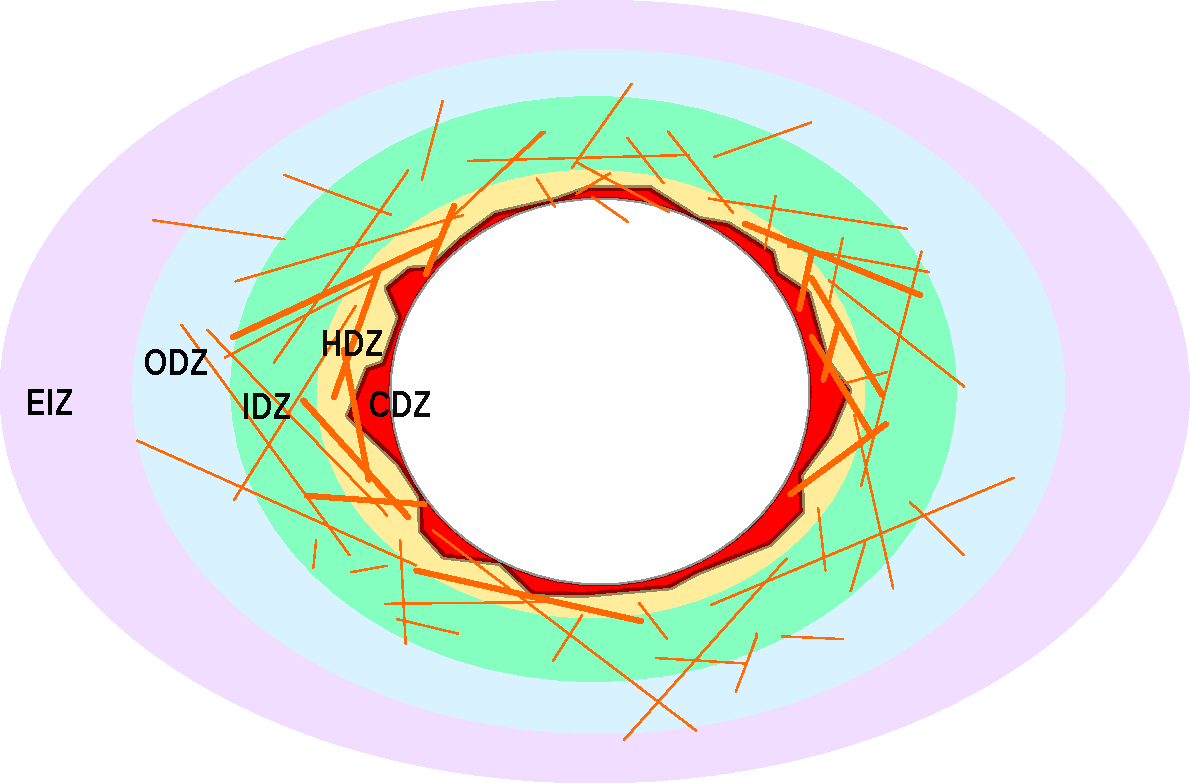
\includegraphics[width=\textwidth]{graphics/EDZ_structure.pdf}
    \caption{Označení zón s kvalitativně odlišnými změnami v důsledku vzniku díla.}
    \label{fig:edz_zones}
\end{figure}

V projektu nebudeme uvažovat zónu CDZ. V případě použití razícího stroje (TBM) je rozsah této zóny zanedbatelný (okolo 1cm), v případě 
ražby střílením je rozsah CDZ významný (až 1m), ale je prakticky nemožné ho predikovat modelem. Charakterizaci CDZ je případně nutné provést in-situ.
Zbylé zóny vznikají v důsldku změny okrajové podmínky na stěně díla. Pro jejich vznik jsou klíčové procesy ve dvou různých škálách. V měřítku rozměru 
díla probíhá hydro-mechanický proces redistribuce napětí a mimo EIZ se jedná o nevratné plastické změny. Ty však jsou v případě křehkých hornin
způsobeny nelineárními procesy na mikro puklinách, kde dochází k překonání třecích sil mezi stěnami nebo porušení jejich výplní. 
Změny v rozevření puklin pak způsobují změny porozity a hydraulické vodivosti. 

Mikroskopický model a určení homogenizovaných parametrů EDZ byde diskutováno v následující kapitole.
V táto kapitole se zaměříme na možné makroskopické modely se zahrnutím plasticity a porušení materiálu.
Nejprve v popíšeme scénář a geometrii úlohy, následně stručně představíme hierarchii modelů se zvyšující složitostí
a v dalších sekcích pak popíšeme tyto modely podrobněji.

\subsection{Konceptuální model ražby}
Uvažujeme válcovou oblast $\Omega$ sahající do vzdálenosti $R$ od osy vyříznutího úložného vrtu o poloměru $r$, délku oblasti označme $L$. Orientačnní rozměry jsou $R\approx 10m$, $r\approx 2m$, $L\approx 1m$. V případě homogenního materiálu lze využít symetrii vzhledem k posunutí podél osy vrtu a uvažovat výpočet pouze ve 2d řezu. Pro zahrnutí vlivu nehomogenit je nutný plný 3d výpočet. Na této oblasti uvažujeme následujícíc scénář:

\begin{enumerate}
\item {\bf Počáteční stav.} Počáteční tenzor napětí $\sigma_0$, viz. sekce \ref{sec:sigma0}, nulové posunutí, hydrostatický tlak.
                       
\item {\bf Po vyražení.} Na stěně vrtu změna okrajové podmínky z nulového posunutí na nulovou tečnou sílu a 
                         atmosférický tlak. Vnější okrajová podmínka nulové posunutí, hydrostatický tlak.
                         Nutno uvažovat nelineární mechaniku a modely poškození v blízkosti tunelu.                    
                         
\item {\bf Po zatopení.} Změna okrajové podmínky na stěně vrtu na hydrostatický tlak, případně tlak bentonitu. 
                        Menší změna, lze uvažovat jednodušší mechanický model.
\end{enumerate}
Výsledkem makroskopického modelu má být rozložení napětí a deformace po ražbě a po zatopení. Pro výpočet budou použity 
parametry konstitutivních vztahů určené pomocí mikro modelu, viz. sekce \ref{sec:micro_EDZ}. 


Vlivem přítomnosti podzemní vody a relativně malé hydraulické vodivosti krystalických hornin dochází k redistribuci napětí 
postupně v horiznotu asi jednoho roku. To je z hlediska stanovení vlastností EDZ po zatopení zanedbatelé a je tedy možné uvažovat 
pouze stacionární hydro-mechanickou úlohu. Nicméně plný hydro-mechanický model relaxace napětí lze pro stanovení vlastností EDZ (viz. Sekce \ref{sec:experiment}).







\subsection{Přehled kontinuálních modelů} 

Pro výpočet poškození hornin je vhodné uvažovat hierarchii modelů \cite{Blaheta2013a}, se zvětšující se složitostí a také různou potřebou vstupních parametrů:
\begin{enumerate}[(i)]
	\item \label{mod_elast} {\bf Elastický model.} Elastický výpočet napětí a deformací a následně indikace, kde dochází k porušení materiálu podle vhodného pevnostního kritéria.
	\item \label{mod_plast} {\bf Plastický model.} Výpočet napětí a deformací za předpokladu, že nemůže dojít ke stavům za mezí platnosti vhodného pevnostního kritéria (plastické modely). Lze uvažovat procesy s postupným zatěžováním a monotónní odezvou (deformační teorie plasticity) i modely se zatěžováním a odlehčováním a trvalými (plastickými) deformacemi,
	\item \label{mod_damage} {\bf CDM} (continuum damage mechanics). Výpočet napětí a deformací za předpokladu, že nemůže dojít ke stavům za mezí platnosti vhodného pevnostního kritéria a zároveň dochází k oslabení (porušování -  damage) materiálu. V případě samotné damage mechanics se neuvažují nevratné deformace.
	\item \label{mod_irev_cdm} {\bf Kombinované modely.} V praxi existuje řada kombinací výše uvedených modelů. Jednak lze uvažovat kombinaci plasticity a damage mechanics, která uvažuje jak oslabení, tak i trvalé deformace. Existuje však také mnoho ad-hoc přístupů, které uvažují postupné oslabování materiálových konstant, viz např. \cite{Perras2016}, \cite{Carranza-Torres1999}.
\end{enumerate}
U modelů \eqref{mod_elast} a \eqref{mod_plast} máme většinou řadu informací o existenci a jednoznačnosti
řešení, o stabilitě, tedy spojité závislosti řešení na vstupních datech, o chybě vznikající  při  diskretizaci  úloh  a  pod.  Složitější je porozumění  modelům CDM, pro které existuje závislost diskretizovaných  modelů na  síti, nejednoznačnost řešení  apod. Proto jsou navrženy CDM modely s regularizací nebo s nelokální definicí deformací a napětí.



\subsection{Elastický model}

Základním modelem pro výpočet napětí a deformací je lineární elasticita s tenzorem malých deformací a Cauchyovým tenzorem napětí, která je popsána trojicí posunutí $\vc u$, deformace $\eps$ a napětí $\sigma$ a vzájemnými vztahy, které platí ve výpočetní oblasti $\Omega$:
\begin{align*}
	- \div(\sigma) &= \vc f &\mbox{v} \ \Omega, \\
	\sigma &= \tn C : \eps + \sigma_0 + p\tn I  &\mbox{v} \ \Omega, \\
	\eps(\vc u) &= (\nabla \vc u + (\nabla \vc u)^\T &\mbox{v} \ \Omega.
\end{align*}
Výše, $\vc f$ vyjadřuje hustotu objemových sil, $\tn C$ je elastický tenzor pružnosti, $\sigma_0$ je počáteční napětí a $p$ pórový tlak vody. 
Dále na hranici $\partial \Omega$ musíme zadat vhodné okrajové podmínky. --

V uvedené formulaci jsou kompresní deformace a normálová napětí v tlaku záporná (mechanická konvence). 
Hlavní napětí (vlastní čísla $\sigma$) pak ozačíme $\sigma_3 \geq \sigma_2 \geq \sigma_1$.
Pro popis pevnostních veličin se ale v geotechnice užívá opačná konvence, kdy normálová napětí v tlaku jsou kladná (geomechanická konvence).
Potom budeme uvažovat hlavní napětí $\sigma_3 \leq \sigma_2 \leq \sigma_1$, kde $\sigma_1$ je největší hlavní napětí, které je obvykle kladné v tlaku.


\subsubsection{Pevnostní kritéria}
Pevnostní kritéria vychází z vypočteného napětí, případně deformace. Přípustné stavy je možné popsat nerovností
$$
	F_s = F_s(\sigma, \varepsilon) \leq 0.
$$
Kritérii často používanými v mechanice hornin jsou Mohrovo-Coulombovo a  Hoekovo-Brownovo  kritérium, viz např. 
\cite{Desai1984}, \cite{Goel2011}, \cite{Zang2010} a \cite{Brady2006}. Tato kritéria nyní popíšeme za předpokladu isotropní horniny.
\begin{itemize}
	\item Mohrovo-Coulombovo kritérium
		$$
			F (\sigma, x) = |\tau| - (c + \sigma_n \mbox{tg} (\phi)) ,
		$$
		kde $\tau$ a $\sigma_n$ je smykové a normálové napětí působící na libovolnou plochu procházející bodem x, $c$ je koheze a $\phi$ je úhel vnitřního tření.
	\item Mohrovo-Coulombovo kritérium lze také vyjádřit pomocí hlavních napětí. Kritické napětí se týká plochy, která je rovnoběžná se směrem prostředního hlavního napětí. Pokud její polohu vyjádříme úhlem $\beta$ mezi normálou a směrem $\sigma_1$, potom na ni budou působit napětí
		$$
			\sigma_n = \frac{1}{2}(\sigma_1 + \sigma_3 ) + \frac{1}{2}(\sigma_1 - \sigma_3 )\cos 2 \beta, \quad \tau = \frac{1}{2}(\sigma_1 - \sigma_3 ) \sin 2 \beta.
		$$
		Kritický poměr pak nastane pro $\beta =  \frac{\pi}{4} + \frac{\varphi}{2}$. Pro tento úhel dostaneme
		$$
			F(\sigma,x) = (\sigma_1 - \sigma_3 ) - \frac{2c\,\cos \phi}{1-\sin \phi} - \frac{2\sin \phi}{1-\sin \phi} \sigma_3 .
		$$
		Kritérium lze také vyjádřit vztahem
		$$
			F(\sigma, x) = (\sigma_1 - \sigma_3) - (q_{cmass} + A\sigma_3) \leq 0
		$$
		kde $q_{cmass}$ je jednoosá pevnost v tlaku (UCS) pro masiv, $q_{cmass} = 2c \cos \phi / (1-\sin \phi)$ a $A = 2 \sin \phi / (1-\sin \phi)$. UCS lze interpretovat jako Uniaxial Compressive Strength (značí se obvykle $\sigma_c$), nebo Unconfined Compressive Strength ($q_c$). Lze také využít pevnost v tahu (tensile strength $\sigma_t$),
		$$
			q_{cmass} = \sigma_c = \frac{2c \cos \phi}{1-\sin \phi}, \quad \sigma_t = \frac{2c \cos \phi}{1+ \sin \phi}.
		$$
		Další možností je vyjádření kritéria ne pomocí hlavních napětí, ale pomocí invariantů napětí. Viz např. \cite{Desai1984}.
	\item Mohrovo-Coulombovo kritérium bývá také doplněno podmínkou žádného či částečného nepřipuštění tahových napětí, tension cut-off.
	\item Hoekovo-Brownovo kritérium je možno považovat za zobecnění Mohrova-Coulombova kritéria. Toto zobecnění bylo určeno empiricky a zohledňuje kvalitu hornin s 						uvažováním jednoosé pevnosti v tlaku (UCS) pro neporušenou horninu $q_c$ na jedné straně, ale parametry charakterizující kvalitu (porušenost) hornin, na straně druhé. 					Kritérium má tvar
		$$
			F(\sigma,x)=(\sigma_1 - \sigma_3 ) - q_c \left[m_b \frac{\sigma_3}{q_c} + s \right]^a ,
		$$
		kde $q_{c}$ jednoosá pevnost v tlaku neporušených kusů horniny, $m_b$ je nelineární parametr závisející na typu horniny, $a$ je parametr rozpukání horniny.
\end{itemize}

\subsection{Plastické modely}
\alert{Perfektně} plastický model je ve tvaru
\begin{table}[ht]
	\centering
	\begin{tabular}{ll}
		\hline
		rozklad tenzoru deformace & $\varepsilon = \varepsilon^e + \varepsilon^p$\\
		Cauchyho napětí & $\sigma = C : \varepsilon^e$\\
		\alert{plastické kritérium} & \alert{$f_p(\sigma)\leq0$}\\
		plastický potenciál & $g_p,\;\;$ \alert{pro asociovanou plasticitu platí} $\partial g_p/\partial \sigma = \partial f_p/\partial \sigma$  \\
		plastické tečení & \alert{$\dot{\varepsilon}^p = \dot{\gamma}(\partial g_p/\partial \sigma), \dot\gamma \geq 0$,}\\
		podmínka duality & $\dot{\gamma} f_p =0$\\
		\hline
	\end{tabular}
\end{table}

\begin{itemize}
	\item V případě Mohrovy-Coulombovy plasticity máme
	\begin{eqnarray*}
		f_p(\sigma) &=& \frac{1}{2} (\sigma_1 - \sigma_3) + \frac{1}{2} (\sigma_1 + \sigma_3)\sin \phi - c \cos \phi, \\
		g_p(\sigma) &=& \frac{1}{2} (\sigma_1 - \sigma_3) + \frac{1}{2} (\sigma_1 + \sigma_3)\sin \psi,
	\end{eqnarray*}
	\alert{kde $\psi$ úhel dilatace (dilation angle), viz \cite{Neto2011}. Poznamenejme, že pro $\phi = \psi$ platí $\partial g_p/\partial \sigma = \partial f_p/\partial \sigma$, a tedy se jedná o asociovaný model. Dále, plastické kritérium $f_p(\sigma)\leq0$ je ekvivalentní s výše uvedeným kritériem, což odvodíme přenásobením funkce
	$F(\sigma, x) = (\sigma_1 - \sigma_3) - \frac{2c\cos \phi}{1-\sin \phi} - \frac{2\sin \phi}{1-\sin \phi} \sigma_3$ výrazem $\frac{1}{2}(1 - \sin \phi)$.}
	\item Místo Mohrovy-Coulombovy plasticity lze také použít Druckerův-Pragerův model, jehož popis i vztah k parametrům Mohrovy-Coulombovy plasticity lze najít v \cite{Neto2011}. 
	\item Plasticita, vycházející z Hoekova-Brownova kritéria je málo obvyklá, ale možná. Viz např. \cite{Carranza-Torres1999}.
\end{itemize}


\subsection{Modely s poškozením}
Samotné modely plasticity neuvažují oslabení materiálu při křehkém porušení. K tomu účelu můžeme zavést parametr oslabení (damage parametr) $\omega\in[0,1]$, kde $\omega = 1$ odpovídá neporušenému materiálu a $\omega = 0$ znamená zcela porušený materiál. Nejjednodušší kombinace elasticity a porušení by potom využívala vztahy
\begin{table}[h!]
	\centering
	\begin{tabular}{ll}
		\hline
		zobecněný Hookeův zákon & $\sigma = (1-\omega)C : \varepsilon$\\
		vývoj porušení & $\omega = g(\kappa), \dot{\kappa} \geq 0, \kappa(0) = \overline{\varepsilon}_0$\\
		funkce porušení & $f_d(\varepsilon,\kappa)=\overline{\varepsilon}(\varepsilon)-\kappa$\\
		podmínka přípustnosti & $f_d(\varepsilon,\kappa)\leq 0$ \\
		podmínku duality & $\dot{\kappa} f_d =0$\\
		\hline
	\end{tabular}
\end{table}

Výše $\overline{\varepsilon}(\varepsilon)$ představuje ekvivalentní tahovou deformaci
$$
	\overline{\varepsilon}(\varepsilon) = (\langle\varepsilon_1\rangle^2+\langle\varepsilon_2\rangle^2+\langle\varepsilon_3\rangle^2)^{1/2},
$$
kde $\langle\varepsilon_i\rangle$ značí absolutní hodnotu tahových hlavních deformací, deformace v
tlaku se neuvažují. Všimněme si souvislosti s pevnostními kritérii využívajícími deformace, přehled lze nalézt v (Kwasniewski, Takahashi 2010). Parametr porušení se vyvíjí v závislosti na zavedené ekvivalentní tahové deformaci. Funkci $g$ můžeme volit exponenciálně s adaptací na diskretizační parametr.

Modelování porušení (Continuum Damage Mechanics) je poměrně složité, viz např. \cite{Lemaitre1992}, \cite{Neto2011}. Proto pouze zmíníme některé složitější podrobnosti:
\begin{itemize}
	\item porušení nemusí být isotropní a může být také odlišné pro namáhání v tlaku a tahu,
	\item v reálných případech se při porušení objevují trvalé deformace, takže
	použijeme opět dělení deformací $\varepsilon=\varepsilon^e + \varepsilon^p$, $\overline{\sigma} = C : \varepsilon^e$, $\sigma = (1-\omega)\overline{\sigma} = C : \varepsilon^e$. Navíc propojíme růst poškození s přírůstkem plastické deformace, $\dot{\kappa} = \|\dot{\varepsilon}^p\|^2 = \dot{\varepsilon}^p : \dot{\varepsilon}^p$.
	\item modely poškození je nutné stabilizovat pro zamezení závislosti na diskretizaci.
\end{itemize}

















\section{Mikro model vzniku EDZ}
\label{sec:micro_EDZ}
Kromě zóny mechanického poškození horniny dochází vlivem odčerpávání podzemní vody ke změně hydraulických poměrů ve větším okolí díla nazývaném zóna ovlivnění (excavation disturbance zone). Díky kontaktu s atmosférou v bezprostředním okolí stěny díla dochází k chemickým změnám, které mohou ovlivnit zejména difúzní a sorpční vlastnosti horniny. Tyto jevy nebudou ve výsledné metodice uvažovány, ale pro výsledné použití je třeba posoudit jejich vliv na výsledky modelu.



Cílem modelu EDZ je predikce vlastností porušené horniny v okolí úložného vrtu ve finálním 
zatopeném stavu za předpokladu znalosti vlastností horniny před ražbou vrtu. 
Zejména nás zajímá predikce tenzoru hydraulické vodivosti $\tn K(\vc x)$ 
a jeho prostorová změna v rámci EDZ a dále transportní parametry: 
koeficient difúze $d$, podélná disperzivita $\alpha_L$ a příčná disperzivita $\alpha_T$. 
Omezíme se pouze na změny v zóně poškození vzniklé změnou napěťových poměrů v hornině 
v důsledku ražby. Zejména nebudeme uvažovat poškození způsobené přímo v důsledku ražby 
(construction damage zone).
Jako nejšetrnější se totiž jeví použití (tunnel boring machine - TBM) 
a v tomto případě je dle \cite{Vavro2016} poškození v důsldku ražby 
do hloubky cca 30mm od stěny díla. 
Vliv teploty na vodivost EDZ může být významným faktorem, ale není uvažován pro zachování 
relativní jednoduchosti modelu. Dále nebudeme uvažovat případné změny hydraulické vodivosti 
EDZ v důsledku chemických procesů. A konečně nebude uvažována žádná metoda sanace EDZ 
(např. různé druhy tlakové penetrace). Cílem je tedy predikce vlastností EDZ se 
zahrnutím vlivu změn napětí a to jak změny v důsledku ražby tak změny v důsledku uzavření 
(zatopení a bobtnací tlak bentonitu).

\subsection{Modely poškození a predikce vodivosti}
Tato kapitola shrnuje možné přístupy k predikci vodivosti EDZ vlivem mechanických změn. Podkladem byl zejména přehledový článek \cite{Shahbazi2020a} na podobné téma. 

Mechaniku lze chápat jako víceškálový model, kde na mikro (mezo) škále je kontinuum rozpukané a velká napětí vedou preferenčně k deformacím a smykům na puklinách případně k jejich propojování. Pro predikcu vodivosti je třeba tyto jevy popsat nad rámec homogenizovaných empirických vztahů pro nelineární mechaniku.






V této sekci jsou shrnuty práce a modely vzniku EDZ zahrnující hydro-elastické modely, modely plasticity, pevnostní kritéria a modely poškození. Výsledkem těchto modelů může být rozsah jednotlivých zón, rozložení napětí a různé míry poškození.



TODO:
- otázka zda je difúze zanedbatelná při malých rychlostech
- zjistit řádově rychlosti na úrovni úložiště
- pro začátek bychom difúzi zanedbali

- klíčový parametr tenzor počátečního napětí
  lze měřit a lze získat 

- výpočet 
- tlak bentonitu 2,5 az 5 MPa, to je zhruba srovnatelne s hg tlakem v 500m cca 5MPa
- Grimsel v zule + teplo, pomala saturace, nebyla saturace ani po 18letech
- 

\subsection{Predikce vodivosti}
Makroskopické modely (Rutquist, Hoek-Brown) využívají různé empirické indexy popisující poškození horniny:

RMR - rock mass rating, RMQ, GSI -

v principu je asi lze nahradit pomocí multiškálového přístupu za předpokladu znalosti 
statistiky mikro puklin.

Dělení na podoblasti dle \cite{Perras2016}, lze založit buďto na 
Hosek-Brown kritériu \cite{}
\cite{Hajiabdolmajid2002}
Možnosti predikce:
\begin{enumerate}
    \item {\bf EIZ - elastický režim} Dokonale vratné malé i velké deformace, pouze změna porozity a tedy změna vodivosti dle Carman-Koženého.
    \item {\bf EDZ - plastický režim} Nevratné změny, vznik drobných poruch, které nelze rozlišit na modelech v měřítku průměru chodby, elementy cca do 1cm. 
    
    Lze použít empirické vztahy \cite{Rutqvist2009} závislosti na deformaci nebo napětí. Dále vztahy závislosti na Rock Mass Rating (z jader) \cite{Liu1999}. Případně jiné. 
    Asi použitelná první možnost, pokud se provede nějaká kalibrace pomocí vhodného měření in situ. \todo{další empirické nelineární vztahy mezi napětím a vodivostí, kalibrované pomocí 
    např. DFN modleu REV (zjednodušený víceškálový přístup).}
    \todo{Podrobněji popsat, uvést odkazy.}
    
    
    Lze uvažovat víceškálový model (snad možno zachytit vznik poruch do velikosti 1um). Na čtverci (1x1cm) uvažujeme náhodné pole mechanických parametrů (elastický tenzor a plastická kritéria). Plastická oblast detekována makro modelem, na ní provedena detailní analýza mikro výpočtem, aplikujeme příslušné pole deformace z makro modelu, v jednoduchém případě počítáme opět plastický model, případně na základě výsledků vygenerujeme nové pukliny a opakujeme výpočet. Následně určíme ekvivalentní tenzor vodivosti. Případně lze průměrovat přes více realizací, resp. lze získat populaci hodnot pro samplování v makro modelech transportu. 
    
    Zde by bylo výhodou, že parametry plastických modelů lze snad určit laboratorně na odvrtaných nepoškozených vzorcích.
    
    \item {\bf HDZ - makro poruchy, propojené} 
    Dle \cite{Perras2016} lze detekovat i tuto zónu plastickým modelem. Je otázkou zda ji je nutné uvažovat, jednak se předpokládá šetrný způsob ražby, ideálně pomocí TBM. Dále lze snad tuto zónu   
    
    Závislost vodivosti na deformaci (Kožený), dále závislost na napětí (Rutqvist), nutno fitovat empirické konstanty pomocí experimentu. 
\end{enumerate}


Hydraulická vodivost $K$ $[m/s]$ je vztažena k permeabilitě $\kappa$ $[m^2]$:
\[
    K =\frac{\kappa \rho g}{\nu}.
\]
pro tekutinu o hustotě $\rho$ $[kg\, m^{-3}]$ a hydrodynamické viskozitě $\nu$ $[s^-1]$.

{\bf Závislost permeability na geometrii.} Pro systémy paralelních nezávislých puklin odvozen kubický zákon: Snow (1965) \cite{Snow1965}:
\[
    \kappa=\frac{d^3}{12 D},
\] 
kde $d$ $[m]$ je rozevření puklin a $D$ $[m]$ je vzdálenost puklin. Pro složitější systémy puklin byly publikovány různé empirické homogenizace, e.g. \cite{Pouya2011}, další možností je použití více škálového modelu, kde je efektivní vodivost rozpukaného média vypočtena na základě mikro modelu. 
Různé homogenizační techniky pro ekvivalentní vodivost směsi materiálů jsou shrnuty v Renard 1997 \cite{Renard1997}.
Zde jsou populární DFN (Discrete fracture network) modely. Ovšem zde je opominutý významný příspěvek mikro puklin k celkové vodivosti, proto preferujeme použití continuum-fracture modelu.


Závislost vodivosti na porozitě je dána Carman-Koženého vztahem:

Vavro (2016) \cite{Vavro2016}: Shrnutí zahraničních poznatků o vzniku a vývoji EDZ v krystalických horninách. Komplexní rešerše k tématům: definice EDZ, vliv EDZ na bezpečnost, mechanismy vzniku EDZ, metody charakterizace EDZ, přehled experimentálníc dat.

\begin{itemize}
    \item dělení EDZ, definice - pro model nepoužitelné
    \item možné pozitivní vlivy EDZ na bezpečnost \cite{Lanyon2011}: hydraulic cage, sorption surface on new fractures, ventilation of gasses, reduction of local transmissivity??
    \item Zdroje poškození:
    
\end{itemize}




\subsection{Rešerše - přehled souvisejících článků}
{\bf \cite{Shahbazi2020a}}\\
Přehledový článek o různých analytických a numerických modelech 
pro prdikci hydraulické vodivosti rozpukaného prostředí i na základě mechaniky. Z numerických přístupů 
jsou použity převážně DFN (discrete fracture networks) a DEM (distinct element method). 
TODO: projiít odkazy, hledání multiscale přístupu, jednoduchý model pro jemnou škálu s puklinami, 
efektivní parametry pro makro škálu

\noindent{\bf \cite{Blaheta2013}}\\
TH model pilíře v laboratoři \"Asp\"o se zahrnutím plasticity a modelů poškození. 
Kalibrace na některé měřené veličiny.



\noindent{\bf \cite{Perras2016}}\\
Použití DISL - damage initiatin and spalling pro predikci hloubky jednotlivých částí EDZ,
porovnání numerických modelů a empirických dat, fitování empirického vztahu pro relativní hloubku 
($r/R$) v závislosti na maximálním tečným napětím na stěně normalizovaném na CI (crack initiation napětí)
,$\sigma_{max} / \sigma_{CI}$. To je nelineární rozšíření vztahu navrženého v
\cite{Martin1999} a \cite{Diederichs2007}). 
DISL je založen na Hoek-Brownově kritériu.

\noindent{\bf \cite{Martin1999}}\\
Analýza hloubky poškození v závislosti na napětí a tvaru tunelu, krystalinika, založeno na Hoek-Brown.

\noindent{\bf \cite{Dreuzy2012}}\\
Porovnání DFN s konstantní vodivostí puklin vs. puklin s heterogenní vodivostí (Gaussian distribution, power-law like correlation). Analýza vlivu celkovou vodivost sítě. Pro heterogenní případ pozorováno převážně snížení celkové vodivosti (faktorem 2 - 6). \todo{podrobnější čtení}



\noindent{\bf \cite{Souley2001}}\\
Model poškození a model změny permeability v závislosti na mechanice, vychází z konceptu paralelních puklin \cite{Snow1965}. Zaměřeno na krystalické horniny, neuvažuje namáhání v tahu.  Implementováno v SW FLAC3D (použit v projektu "Hluboké horizonty").

\noindent{\bf \cite{Rutqvist2003}}\\
Přehled HM modelů pro rozpukanou horninu s různými konstitutivními 
vztahy pro explicitní popis vlastností puklin v závislosti ne tečném a normálovém napětí. 
Příklady aplikací a porovnání s měřeními.
Vztah mezi permeabilitou a "confining pressure" 
(pokles vodivosti s hloubkou. Jsou diskutovány vztahy mezi napětím resp. 
porozitou a permeabilitou. Matematický popis jevů na puklinách. Rozdíl mezi "apparent aperture" 
a "real apperture". 



{\bf \cite{Kelsall1984}}:\\
Základní článek zabývající se otázkou změny hydrulické vodivosti v EDZ. 
Odvozeno analytické řešení pro rozložení napětí v okolí ideální kruhové chodby. 
Změny v hydraulické vodivosti jsou dále odvozeny na základě kubického zákona. 
Na základě tohoto modelu predikují zvýšení vodivosti o jeden až dva řády pouze vlivem změny napětí. Změna alespoň o jeden řád nejvýše do vzdálenosti dvou průměrů od stěny chodby. Ražba střílením může dále zvýšit hydraulickou vodivost, avšak jen v blízkosti (cca. 0,3 m) stěny chodby.


{\bf \cite{Lisjak2014}}\\
Modelování vzniku puklin v EDZ pomocí \uv{hybrid finite discrete elements method},
přehled jiných numerických přístupů. 

{\bf  \cite{Barton1985}}\\
Measurement of fracture apperture and "real" apperture used in models.

{\bf \cite{Shao2005}}\\
Mechanické vlastnosti a permeabilita křehkých hornin, vztahy odvozené na základě sítě mikropuklin, zahrnut vliv propojenosti, porovnání s laboratorními experimenty. Asi nejblíže našemu záměru, netriviální formulace mechaniky pomocí mechanické entalpie a nejasné odvození.


\section{Inverzní úlohy a geofyzikální měření}
\subsection{Počáteční napětí}
\label{sec:sigma0}
Počáteční napětí výrazně ovlivňuje výsledné napěťové pole a tím i charakter EDZ.
V horninovém masívu s elastickým chováním a s Poissonovou konstantou $\nu$, v hloubce $h$ a s průměrnou hustotou nadložních hornin $\rho_{r}$ a v případě,
že na horniny nepůsobí jiné vlivy než váha hornin, je počáteční napětí $\sigma_0$
popsáno halvními napětími ve směrech souřadného systému $(\sigma_x, \sigma_y, \sigma_z)$ určenými vztahem
\begin{equation}
	\sigma_z = h\,\rho_{r}\, g, \quad \sigma_x = \sigma_y = \frac{\nu}{1-\nu} \sigma_z,
\end{equation}
přičemž $g$ je gravitační konstanta. Pro hloubku 500 m a $\nu = 1/4$ uvedené vyjádření dává hodnoty
$$
	\sigma_z = 13.5, \sigma_x = \sigma_y = 4.05\quad [MPa].
$$
Reálná počáteční napětí však mohou mít převažující horizontální složky a obecné vlastní vektory (nerovnoběžné se souřadným systémem). Například napětí měřené v hloubce 420 m v Underground Research Laboratory (URL) blízko Lac du Bonnet, Manitoba, Kanada, dosahuje hodnot
$$
	\sigma_3 = 11, \sigma_2 = 45, \sigma_1 = 60\quad [MPa]
$$
viz \cite{Rutqvist2009}. V tomto případě musíme počítat i se smykovými napětími. Počáteční napětí může být velmi proměnné i v rámci jedné lokality, zvláště pokud je navíc ovlivněna více podzemními díly, viz příklad laboratoře GRIMSEL ve Švýcarsku, viz. \cite{Krietsch2019},
\cite{Stas2016}, \cite{Rutqvist2004}. Pro studium EDZ je proto vhodné uvažovat výpočty pro různé hodnoty počátečního napětí.



Poznamenejme  ještě, že počáteční napětí $\sigma_0$, které může být určeno měřením \alert{nebo výpočtem pomocí inverzní analýzy (viz zaslaný článek od J. Malíka),  může být zavedeno do konstitučního vztahu následovně:} $\sigma = C  : \varepsilon + \sigma_0$ v $\Omega$. Obdobně může být do konstitučního vztahu zaveden pórový tlak podzemní vody.


Jelikož cílem projektu je poskytnout predikci indikátorů bezpečnosti 
včetně charakterizace nejistot, je třeba standardní inverzní metody při zpracování geofyzikálních a jiných dat nahradit Bayesovskými inverzními metodami. Bayesovský přístup bude nejprve aplikován samostatně na vybrané druhy dat, která umožní nejlépe identifikovat parametry transportního modelu a modelu EDZ. V této sekci jsou shrnuty práce věnované experimentální charakterizaci EDZ s využitím různých metod.

S ohledem na výslednou permeabilitu zavedeme vlastní rozčlenění EDZ na základě mechanických dějů:
\begin{itemize}
    \item [Damage zone] - dochází k tvorbě nových makroskopických puklin, poškození
    \item [Plastic zone] - plastická (mikro trhliny)
    \item [Elasitic zone] - non-linear elasticity (fracture openning)
\end{itemize}
Není jasné co je v pracech myšleno pojmem "reverzibilní změny", jelikož i elasticky reverzibilní deformace jsou reálně irreverzibilní (nedojde k obnově původního napětí).



Změny v EDZ jsou HM proces a mhou tedy probíhat déle v závislosti na hydraulické vodivosti. Pro vodivost 1e-9 je čas transport na vzdálenost 1m při tlakovém spádu 1m cca 31 let. Reálné relaxační časy budou výrazně kratší, ale určitě v řádu dnů nebo měsíců. 

\section{Identifikace parametrů}
\label{sec:parameters}

Tato kapitola shrnuje měřící techniky, které mohou poskytnout přímou nebo nepřímou informaci 
o fyzikálních vlastnostech EDZ. Zejména nás zajímá charakterizace permeability, puklinových statistik a porozity. Ale i mechanické parametry: modul pružnosti, Poissonovo číslo, anisotropie elastického tensoru,  parametry plasticity ...
Převážně založeno na Vavro (2016) \cite{Vavro2016} a doplněno o méně obvyklá měření.


Možná měření na průzkumných vrtech:
    \begin{itemize}
        \item optická a ultrazvuková karotáž - identifikace protnutých geologických poruch;
        \item elektrická odporová tomografie vůči sousední paralelní chodbě
        \item seismika vůči sousední paralelní chodbě;
        \item tlakové zkoušky v různých úsecích vrtu.
    \end{itemize}

{\bf MWD (Measure While Drilling)} \cite{JeroenvanEldert2018}

{\bf GPR (Ground Penetrating Radar)} 

{\bf ERT (Electrical resistence tomography)}


{\bf Seismicity}

{\bf  Borehole Core Drilling and Logging} \cite{Lanyon2011}

{\bf Mapping of the Excavation Surfaces} \cite{Lanyon2011}

{\bf  Resin Injection and Overcoring} \cite{Lanyon2011}

{\bf  Sonic and Ultrasonic Measurements} \cite{Lanyon2011}
{\bf  Acoustic Emission} \cite{Lanyon2011}

{\bf  Resistivity/Geo-electrical Measurements} \cite{Lanyon2011}

{\bf  Radar Measurements} \cite{Lanyon2011}

{\bf  Hydraulic Characterization} \cite{Lanyon2011}

{\bf  Geomechanical Characterization} \cite{Lanyon2011}

{\bf  Geochemical Characterization} \cite{Lanyon2011}

{\bf MVP - microvelocity probe} \cite{Rutqvist2009} 
{\bf SEPPI - a permeability measurement} \cite{Rutqvist2009} 


\subsection{Rešerše prací}

{\bf Říha et al. (2019)} Task G, TAS04: Dostupná data: 
\begin{itemize}
    \item Geometrie tunelu, mračno bodů.
    \item Počáteční a koncový bod vrtů (celkem 15 z toho 3 vtláčecí a 4 měřící).
    \item Otevřené zóny vrtů (10-20cm, 20-40cm, 40-60cm).
    \item Pukliny odečtené na povrchu tunelu.
    \item Průměrné charakteristiky horniny.
    \item GPR data, identifikované pukliny do hloubky 40cm.
    \item DFN - stochasticaly generated (not clear for which statistical parameters)
    \item Odhadované charakteristiky EDZ jako kontinua.
    \item Overall pressure and stress gradiends in the domain.
\end{itemize}

{\bf Aoyagi and Ishii al. (2018)} \cite{Aoyagi2018}: horní odhad hydraulické vodivosti v EDZ (laboratoř Horonobe, Japonsko) na základě MSI (Mean Stress Index). Model porovnán s měřením z různých metod: průměrné charakteristiky horniny z různých měření, vizuální identifikace puklin v konkrétních vrtech (rozevření nad 0,1 mm), klasifikace puklin v jádrech, měření mechanických posunutí v chodbě, tlakové zkoušky.

{\bf Armand et al. (2014)} \cite{Armand2014}: Charakterizace indukované sítě puklin v EDZ v laboratoři URL (Bure, Francie). Použité metody: 3d sken jader, analýza puklin na jádrech, seismická měření, hydraulické testy a injektáž pryskyřice ve vrtech. 

{\bf Bláha et al. (2017)} \cite{SURAO_184/2014}: přehled geofyzikálních měření na PVP Bukov.
Podrobná zpráva o ERT a seismických měřeních na PVP Bukov, interpretace s předpokládanou hranicí zóny poškození, resp. zóny ovlivnění.  

{\bf Staš a Bláha (2019)} \cite{SURAO_351/2019}: Vznik a monitoring EDZ při výstavbě PVP Bukov.
Podrobná zpráva o dlouhodobém monitorování napětí během vzniku EDZ, identifikace původního napětí v hornině. Celkově rozporuplné výsledky v důsledku velké heterogenity horniny a lokálnímu charakteru metody. Shrnutí ERT a seismických měření, interpretace s předpokládanou hranicí EDZ.  

{\bf Eldert (2018)} \cite{JeroenvanEldert2018}: Charakterizace blast damage for the DaB (drill and blast) method. Využití MWD pro predikci EDZ.

\section{Návrh experimentu pro popis vzniku EDZ}

\label{sec:experiment}
\bibliography{zprava.bib}


\pagebreak


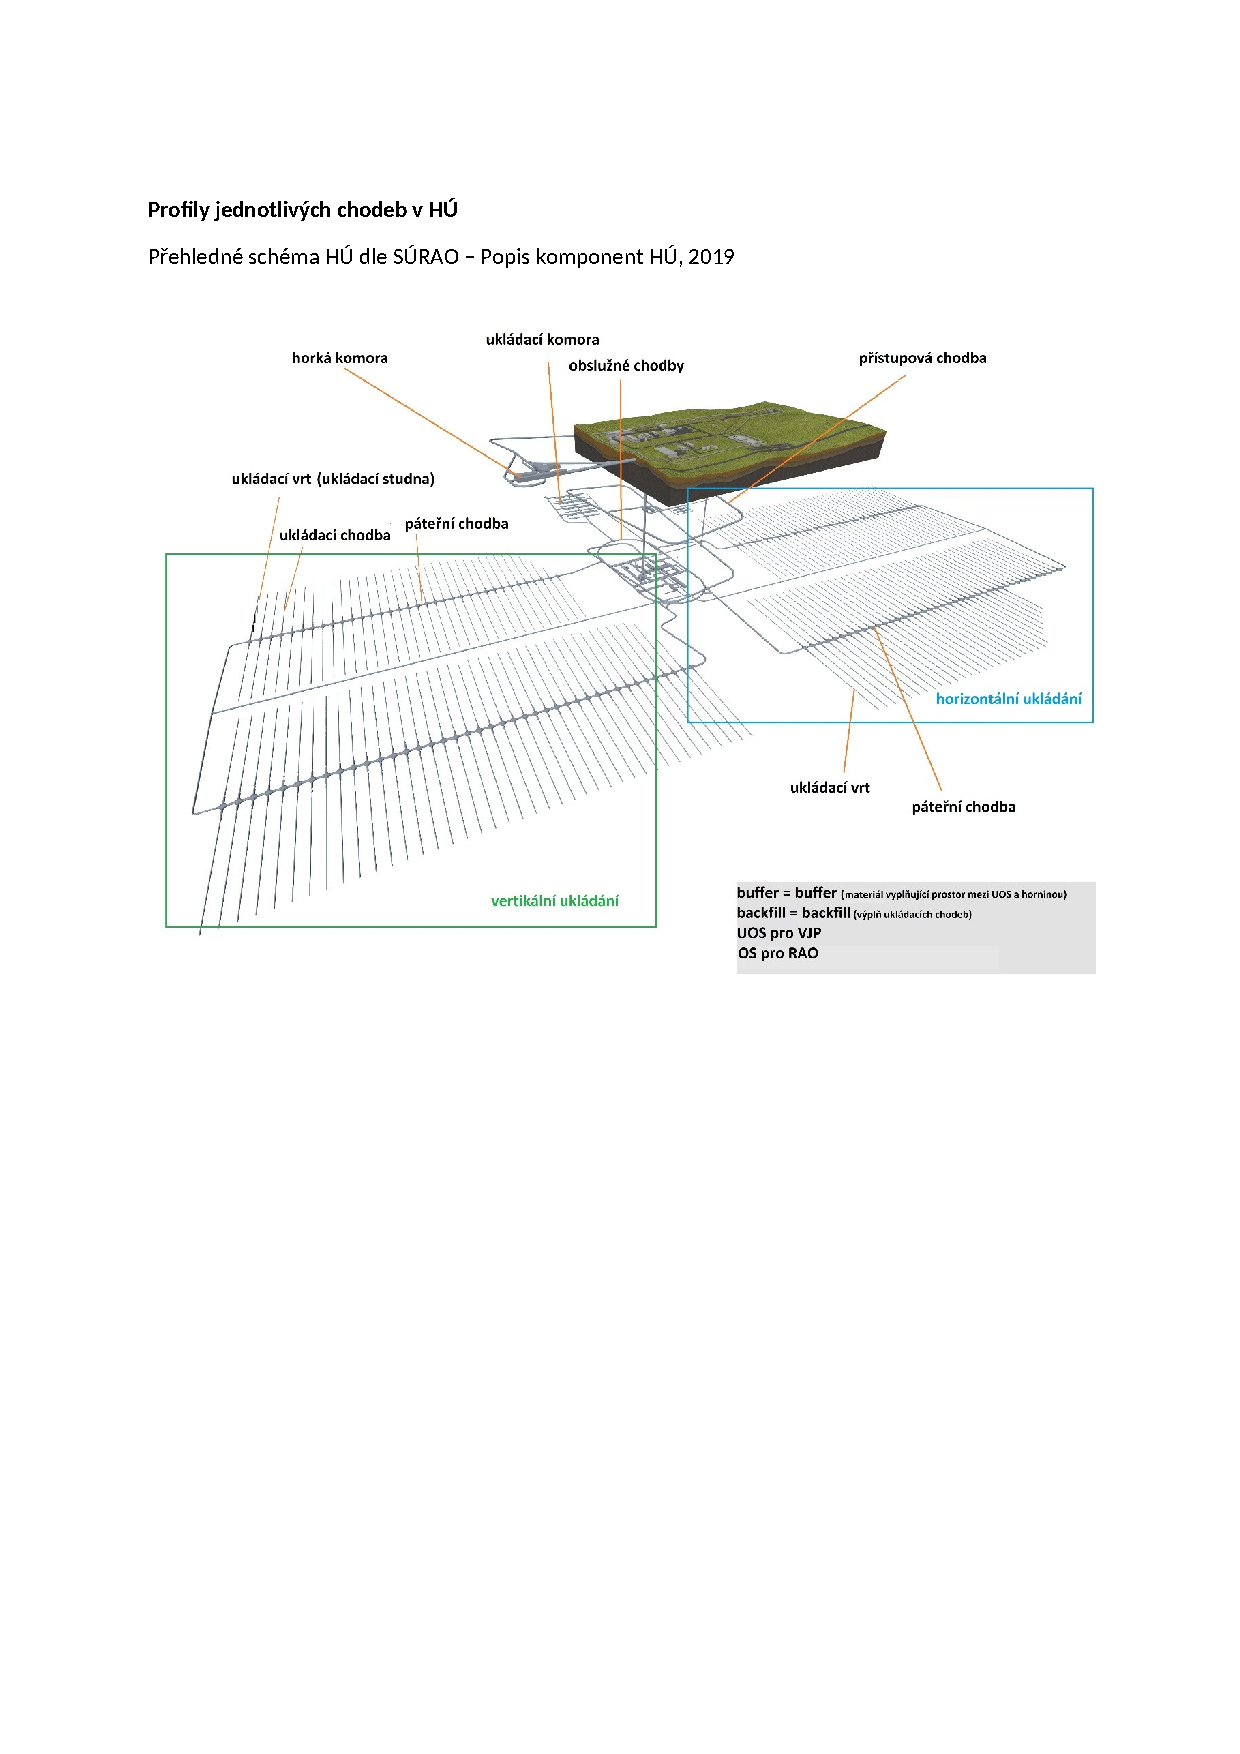
\includepdf[scale=0.99, offset=0 -3cm, page={1},
pagecommand=\section*{Dodatek A - Geometrie HÚ dle SÚRAO}]{Geometrie_HU.pdf}

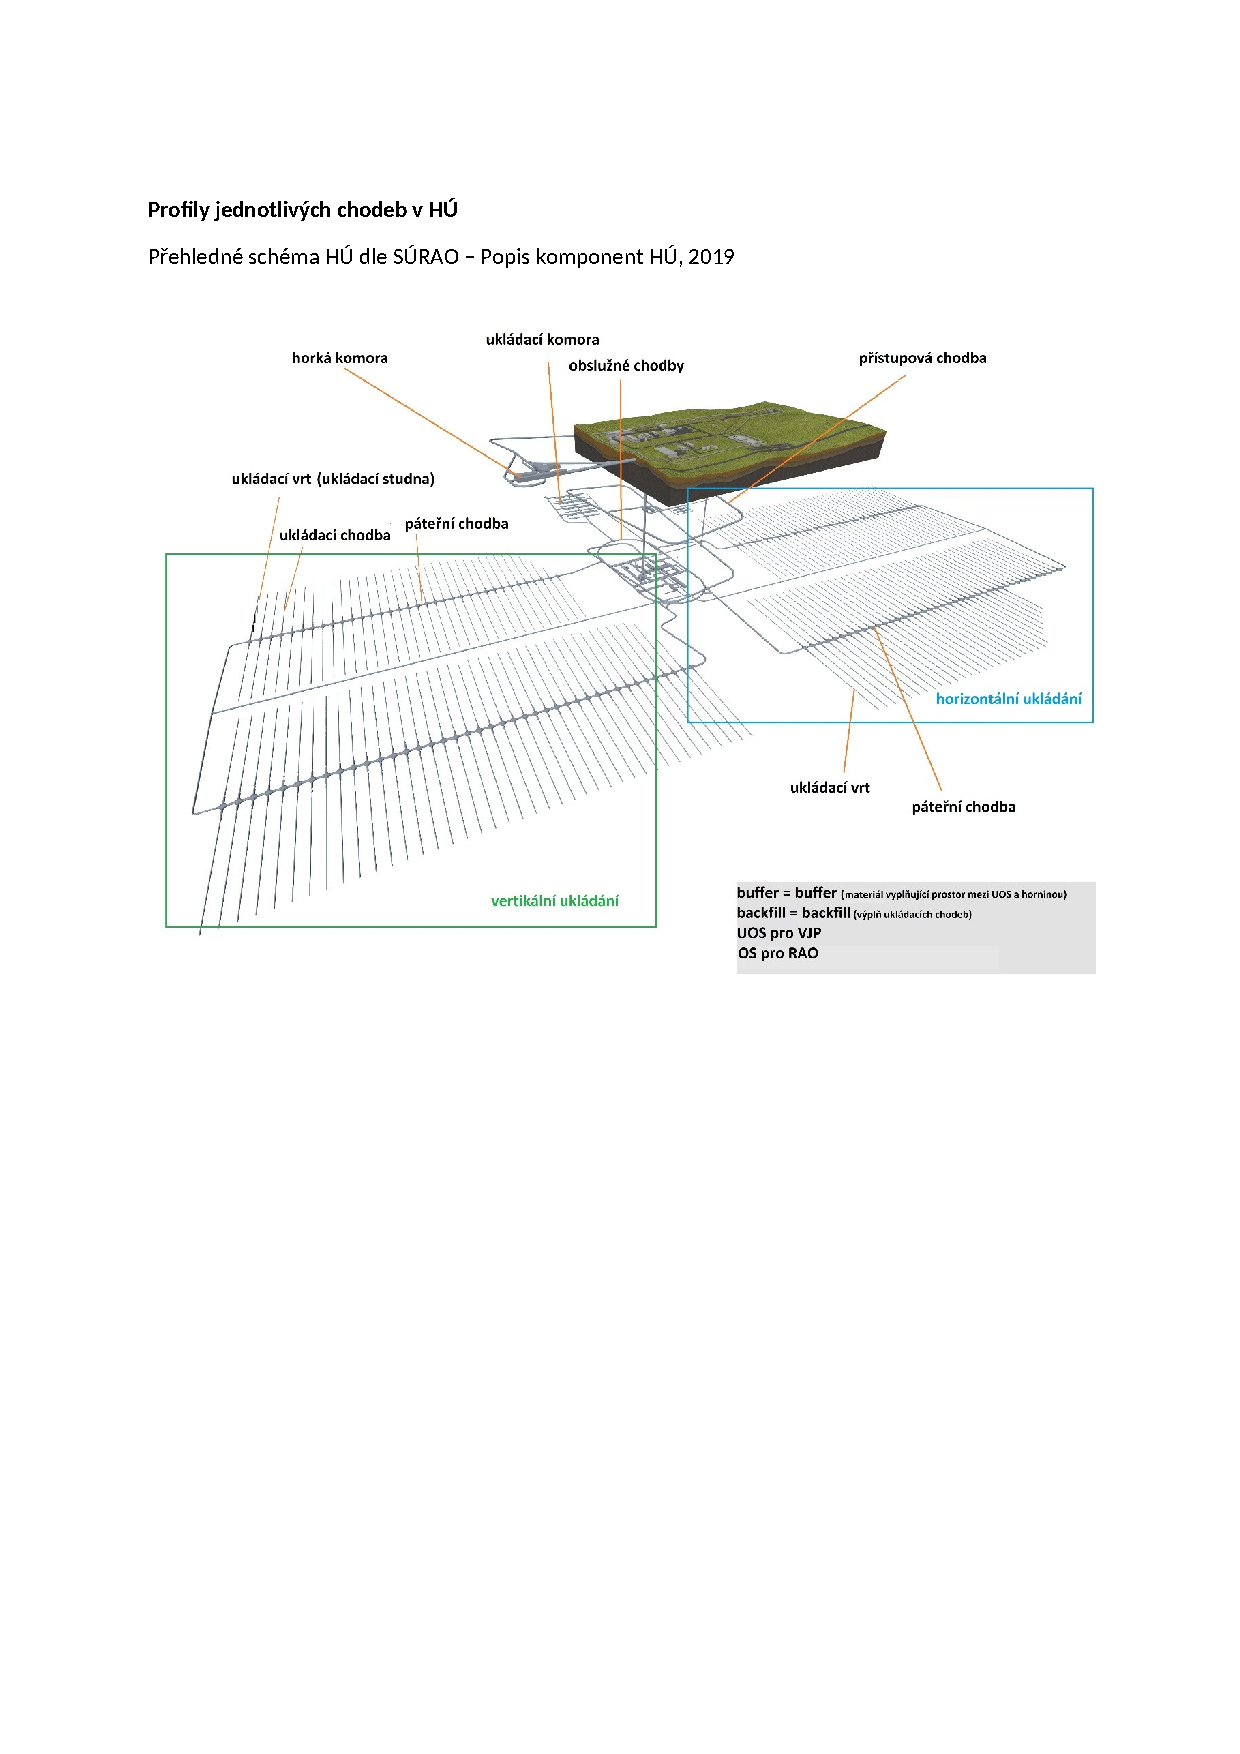
\includepdf[scale=0.99, offset=0 -3cm, page={2,3}]{Geometrie_HU.pdf}

\section*{Dodatek B - odvození řešení rovnice advekce-difúze}
Hledejme nejprve řešení rovnice bez rozpadů na pravé straně:
\begin{equation}
    \label{eq:no_decay_ad}
    R\prtl_t c + v \prtl_x c - d \prtl^2_x c = 0
\end{equation}

pro neznámou koncentraci $c(t, x)$ pro časy $t>0$ a na oblasti $x>0$ s počáteční podmínkou $c(0, x) = 0$ a
okrajovými podmínkami:
\[
    \prtl_t c(t, \infty) = 0,
\]
\[
    c(t, 0) = c_0(t),
\]
kde $c_0 \in C^\infty$.

Analytická řešení a aproximativní řešení uvedené rovnice pro různé druhy počátečních
a okrajových podmínek lze nalézt v \cite{Genuchten1982} (str. 9). 
Speciálně pro případ skokové okrajové podmínky:
\begin{equation}
    \label{eq:jump_bc}
    c_0(t) = \left\{\begin{array}{ll}
         0 & 0 < t < t_0 \\
         1   & t_0 < t
    \end{array}\right. 
\end{equation}
má rovnice řešení:
\begin{equation}
    \label{eq:jump_sol}
    \tilde c(t, x) = 
    \left\{\begin{array}{ll}
         0                     & 0 < t < t_0 \\
         A(t,x)   & t_0 < t,
    \end{array}\right. 
\end{equation}

kde
\[
    A(t,x) = \frac12 \mathrm{erfc}\Big(\frac{ax-bt}{\sqrt t}\Big)
    + \frac12 e^{cx}\mathrm{erfc}\Big(\frac{ax+bt}{\sqrt t}\Big),
\]
\[
    a = \frac{R}{2\sqrt{dR}},\quad 
    b=\frac{v}{2\sqrt{dR}},\quad 
    c=\frac{v}{d}.
\]

Řešení pro obecný průběh okrajové podmínky $c(t,0) = c_0(t)$ lze napsat v konvolučním tvaru:
\[
    c(t,x) = \int_0^t c_0(s) g(t - s, x) ds,
\]

kde jádro $g(t - s, x)$ je řešením rovnice pro okrajovou podmínku $c_0(t) = \delta(t - s)$. 
Tato okrajová podmínka je formálně derivací jednotkového skoku \eqref{eq:jump_bc}. 
Proto jádro bude derivací odpovídajícího řešení:
\[
    g(t, x) = \prtl_t A(t, x) = 
    \frac{1}{2\sqrt{\pi}} 
    e^{-\big( \frac{ax-bt}{\sqrt{t}}\big)^2}
    \Big[ ax t^{-\frac32} + b t^{-\frac12}\Big]
    + \frac{e^{cx}}{2\sqrt{\pi}}  
    e^{-\big( \frac{ax+bt}{\sqrt{t}}\big)^2}
    \Big[ ax t^{-\frac32} - b t^{-\frac12}\Big].
\]
Tento tvar by měl být použitelný i pro numerický výpočet.


Řešení rovnice s rozpadovým členem na pravé straně
\[
 R\prtl_t c + v \prtl_x c - d \prtl^2_x c = - \lambda c
\]
pro stejné okrajové a počáteční podmínky pak nalezneme ve tvaru:
\[
    c(t,x) = U(t,x) e^{-\lambda t},
\]
kde $U(t,x)$ řešením rovnice bez rozpadového členu \eqref{eq:no_decay_ad}, ovšem s okrajovou podmínkou
\[
    \tilde{c}_0(t) = c_0(t) e^{\lambda t}.
\]


% Rovnici vydělíme $R$, označíme
% \[
%     v_r = v/R,\quad d_r = d/R,\quad \lambda_r = \lambda/R.
% \]
% a provedeme transformaci:
% \[
%     c(t, x) = g(t, z),\quad z = \frac{x - v_r t}{\sqrt{d_r}}.
% \]
% Obdržíme rovnici:
% \[
%     \prtl_t g -  \Delta g = - \lambda_r g
% \]
% pro $t>0$, $z > - \frac{v_r t}{\sqrt{d_r}}$, $g(0, z) = 0$, $g(t, \frac{- v_r t}{\sqrt{d_r}}) = c_0(t)$.

% Její řešení má tvar:
% \[
%   g(t,z) = G(t,z) e^{-\lambda_r t}
% \]
% kde $G(t, z)$ je řešení homogenní rovnice:
% \[
%     \prtl_t G -  \Delta G = 0
% \]
% s okrajovou podmínkou $G(t, \frac{- v_r t}{d_r}) = c_0(t) e^{\lambda_r t}$.

% Jádro $\phi(t, z)$ pro 


% \begin{equation}
%     g(t, z) = (4\pi t)^{-\frac12} e^{\frac{-z^2}{4t}} e^{-\lambda_r t},\quad
%     ,
% \end{equation}
% kde jsme označili




\end{document}
